
\documentclass[conference]{IEEEtran}
\IEEEoverridecommandlockouts
% The preceding line is only needed to identify funding in the first footnote. If that is unneeded, please comment it out.
%Template version as of 6/27/2024

\usepackage{cite}
\usepackage{amsmath,amssymb,amsfonts}
\usepackage{algorithmic}
\usepackage{graphicx}
\usepackage{textcomp}
\usepackage{xcolor}
\def\BibTeX{{\rm B\kern-.05em{\sc i\kern-.025em b}\kern-.08em
    T\kern-.1667em\lower.7ex\hbox{E}\kern-.125emX}}
\begin{document}

\title{A Compact, Low-cost Sensor Suite  for Laboratory Experiments
}

\author{\IEEEauthorblockN{1\textsuperscript{st} Bernardo Carvalho}
    \IEEEauthorblockA{\textit{Instituto de Plasmas e Fusão Nuclear} \\
\textit{Universidade de Lisboa, Av. Rovisco Pais 1, 1049-001}\\
\textit{1049-001 Lisboa, Portugal}\\
bernardo.carvalho@tecnico.ulisboa.pt}
\and
\IEEEauthorblockN{2\textsuperscript{nd} Mário Lino da Silva}
\IEEEauthorblockA{\textit{Instituto de Plasmas e Fusão Nuclear} \\
\textit{Universidade de Lisboa, Av. Rovisco Pais 1, 1049-001}\\
Lisboa, Portugal }
\and
\IEEEauthorblockN{3\textsuperscript{rd} Horácio Fernandes}
\IEEEauthorblockA{\textit{Instituto de Plasmas e Fusão Nuclear} \\
\textit{Universidade de Lisboa, Av. Rovisco Pais 1, 1049-001}\\
Lisboa, Portugal }
}

\maketitle

\begin{abstract}
This work describes a new concept in the development of Physics Laboratory experiments and a working prototype, following the Do-It-Yourself (DYI) philosophy,
showing to students that sophisticated experiments may be conducted using off-the-self electronic equipment.
It also provides with an University teaching staff an increased flexibility in preparing and conducting experiments. 
This does not aim to replace traditional laboratory experiments which resort to more sophisticated and dedicated equipment,
but instead to complement such experiments with more simplified experiments that may be setup on an as needed basis.

\end{abstract}

\begin{IEEEkeywords}
Physics, Laboratory Experiments, Remote Control, Online Data.
\end{IEEEkeywords}

\section{Introduction}
% Framework
The availability of widespread, cheap, and relatively powerful electronic devices provides for unique and exciting opportunities for developing flexible, ``off-the-shelf'' laboratory experiments where a suite of diagnostics can be deployed to monitor and instrument generic devices under study.

Besides the ubiquitous, low-level diagnostics available in the laboratory environment (such as multi-meters, or even generic, low cost oscilloscopes), it is now possible to develop very cheap and reliable diagnostic devices to measure quantities such as  
Temperatures, Pressure, Force, Magnetic field, Electric (V,I and R), Movement, Sound, etc (e.g. a kit box with more than 50 sensors can be bought online for $<$ 10€).

In addition to this we now have access to cheap and rugged "embedded computer” solutions, chiefly the Raspberry-Pi, Arduino\cite{b2} and compatible suites.
These allow for a fully customized, dedicated online connected computer capable of handling very reasonable acquisition rates (around 10KHz) 
and delivering the resulting data in electronic form. The experimental data can be upload to open databases and the students can easily retrieve 
 directly to standard generic (e.g. Excel), or more advanced processing tools (MATLAB, Python, etc.)

The main objectives were to develop an open ecosystem with a flexible, low-cost suite of diagnostics with an ``uncomplicated'' interface; ii) capitalize on the significant developments/cost reductions that have taken place in the last decades regarding micro-controllers/microcomputers, and iii)

\section{Architecture}
The hardware backbone for this platform consists in a combination of a Raspberry-Pi (RPi) board computer and an Arduino compatible board. 
The Rpi will host all the developing  apps, communications infrastructure, database server, online servers (apache, Grafana). 
 A cabled Ethernet connection is preferable, but not  required, since the RPi is able to use an Wifi connection, 
 for example using the "Hop-Spot" function on the instructor’s smartphone, also shared to the student’s phones or mobile PCs.

 The experiment sensor's will be connected to an Arduino board, or compatible.
 Most promising and cost effective units presently are the ESP32 micro-controller based devices, in particular the M5Stick-CP2,
 that are fully wireless, since include a battery and connect directly to Wifi.
 %(An example is shown in `Fig.~\ref{figM5}'')

 Two different architectures are envisaged, one Unitary to be used by the instructor during regular classes, and one Multiple (``Fig.~\ref{figMultiple}''),
 where a complete hardware kit is lended to groups/individuals. 
 In both configurations all experimental data is stored in Web-based Time Series Batabase\cite{b3} (TSDB).
 
\begin{figure}[htbp]
\centerline{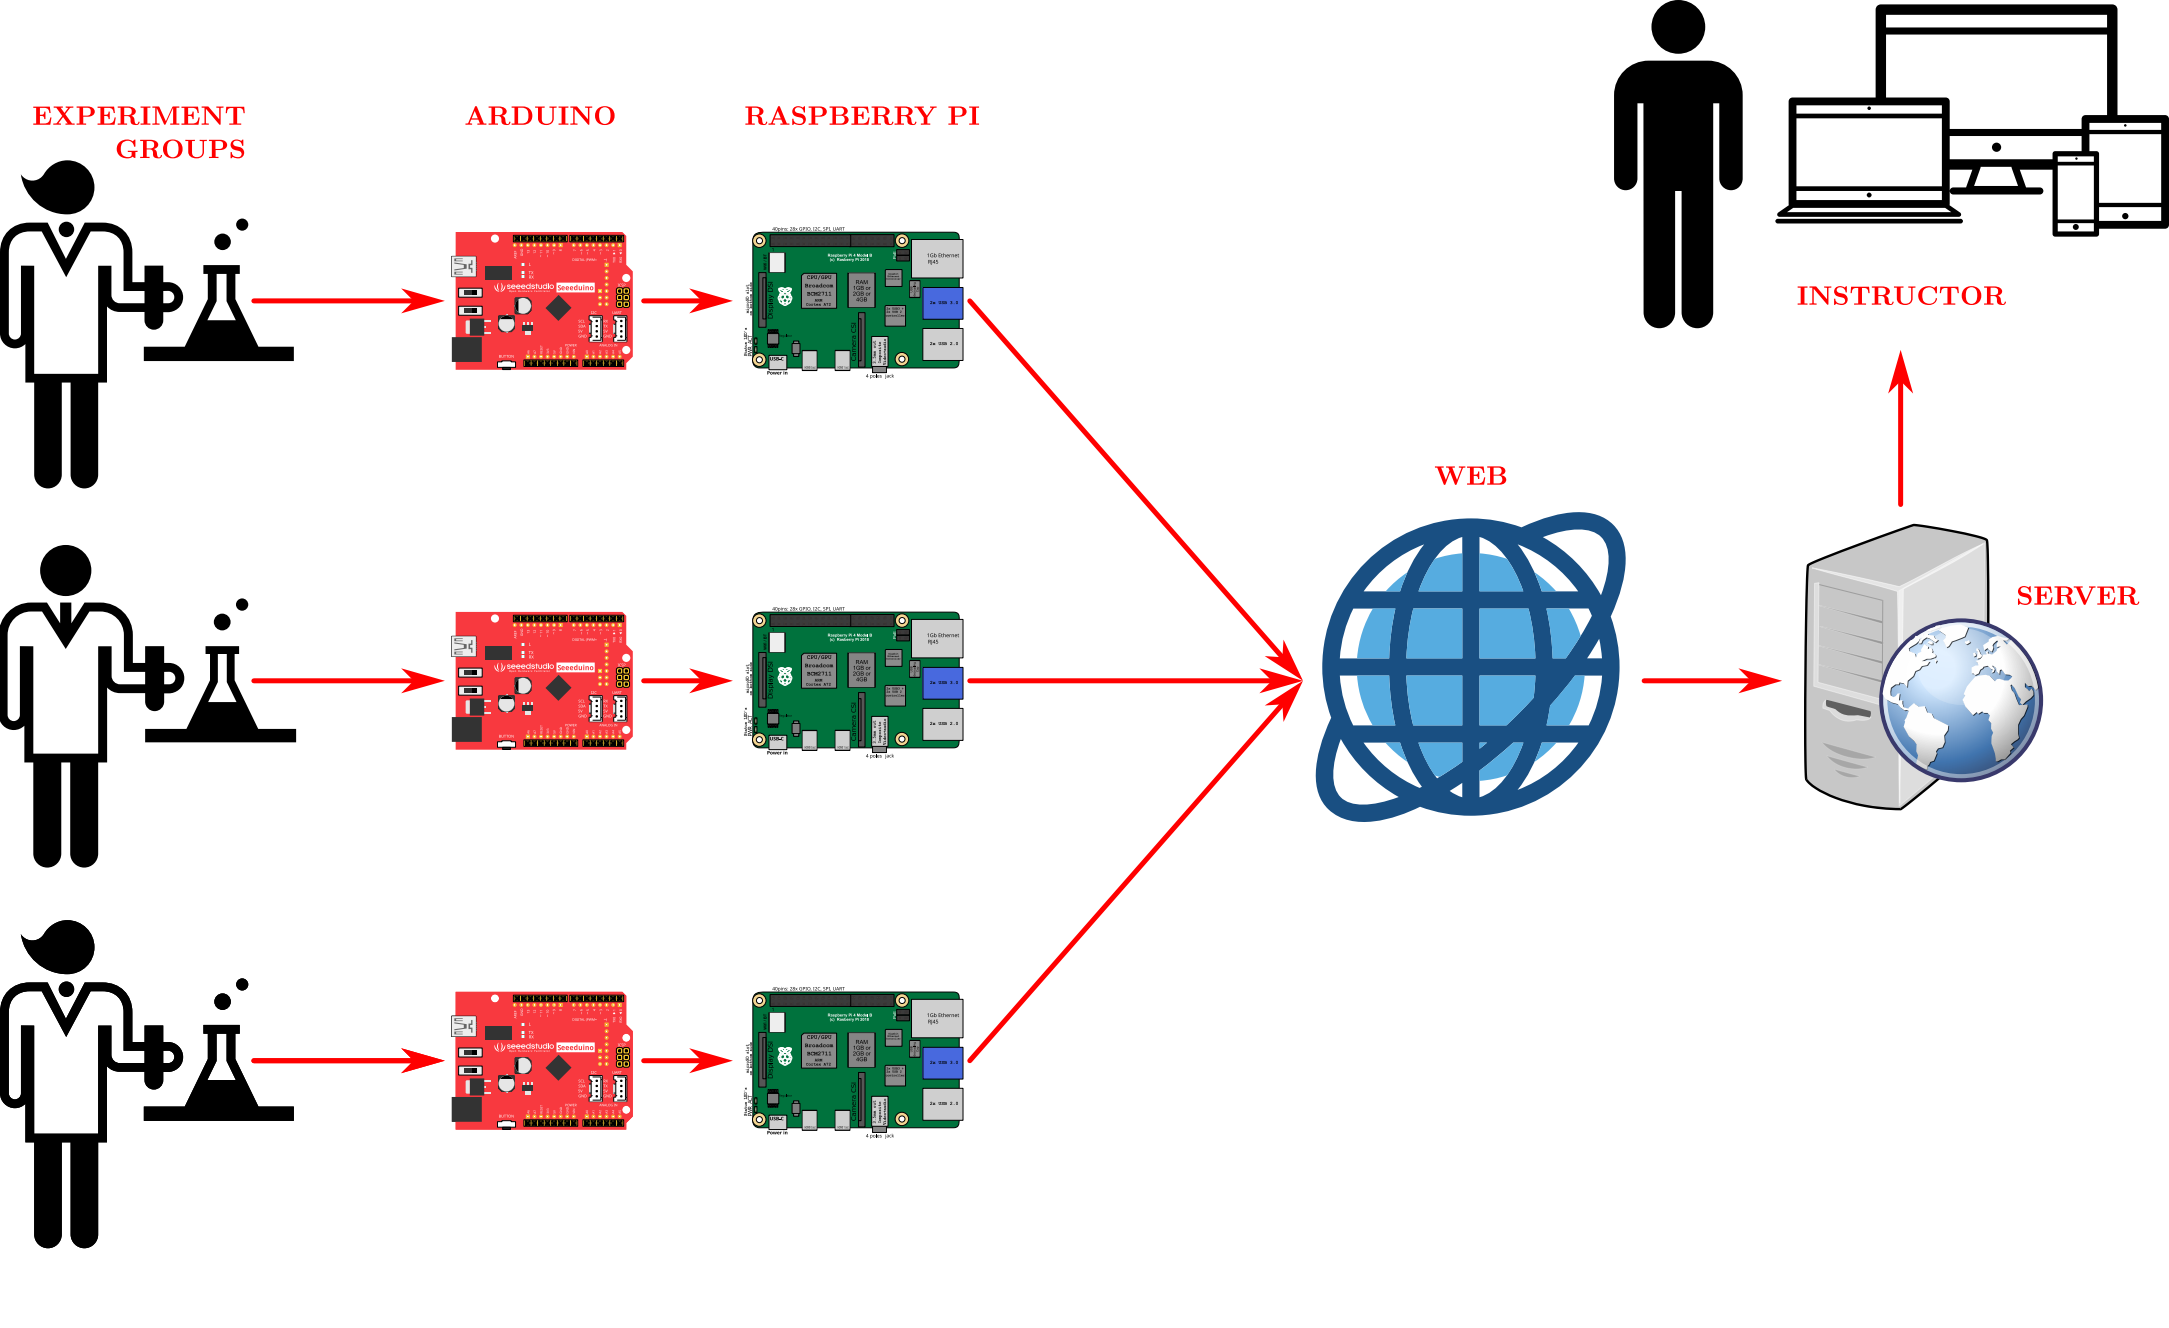
\includegraphics[width=.6\columnwidth]{Multiple.png}}
\caption{Several groups perform the experiment in class and upload the results to a server.}
\label{figMultiple}
\end{figure}

The two computing boards will placed in stackable briefcases used to transport each individual set of experiments.
Each briefcase size is “1 Storage Unit” (1SU), allowing easy and flexible transportation of up to 4-5 sets of experiments with a small trolley.


\section{Applications}
The equipment is to be applied to a very wide range of experiments, ranging from license courses laboratory experiments (fundamental physics), 
to more advanced experiments in master courses. 
But most of all, the equipment is to have robust and well-maintained documentation, 
following the best “Libre” software/hardware practices, encouraging users to come up with novel experiments.

A live library of experiments, with a description of the selected instrumentation, and the associated tailored code will be maintained and made available in a seamless fashion. 
This means for example providing dedicated ISO’s that only require flashing on the Raspberry/Arduino SD cards, after which the diagnostic setup is ready for deployment,
or a more sophisticated option of providing a library of configurations of the chip to be loaded on a case-by-case basis.

Each experiment would have an associated laboratory guide, either in PDF, or wiki form (or both) and one or more Jupyter\cite{j2} Notebooks. 

A dedicated platform for exchange of information/code/documentation/etc... was developed and host on a public Github\cite{gh} repositóry. 
At later stages of the project, after successful proof-of-concept deployments of the sensor suite, more experiment will be added.


\section{Pilot Experiments}
A demo prototype was assembled and already used in Laboratory demonstration section  were concluded at IST (See ``Tab.~\ref{tab1}'').

\begin{table}[htbp]
\caption{List of Pilot Experiments}
\begin{center}
\begin{tabular}{|c|c|c|c|}
\hline
\textbf{Degree}&\textbf{Year}&\textbf{Course} &\textbf{Experiment}\\
\hline
Civil Eng. & 2nd&  Thermodynamics & Calorimetry\\
\hline
Civil Eng. & 2nd&  Thermodynamics & Stirling Engine\\
\hline
 Electric Eng.& 1rst&  Physics (Mechanics) & Maxwell Wheel\\
\hline
\end{tabular}
\label{tab1}
\end{center}
\end{table}

As an example, the Maxwell Wheel is a introductory Physics lab where the student are invited to Wheel's Inertial Momentum  $I_z$,
and perform a long and time consuming measurement series of time and velocity,
in different positions.
Traditionally it is measured  with the help of an optical barrier, that has to be moved in small steps(``Fig.~\ref{figMaxwell}''). 
The triggering device is fragile, often fails which disturb student's attention. 

\begin{figure}[htbp]
    \centerline{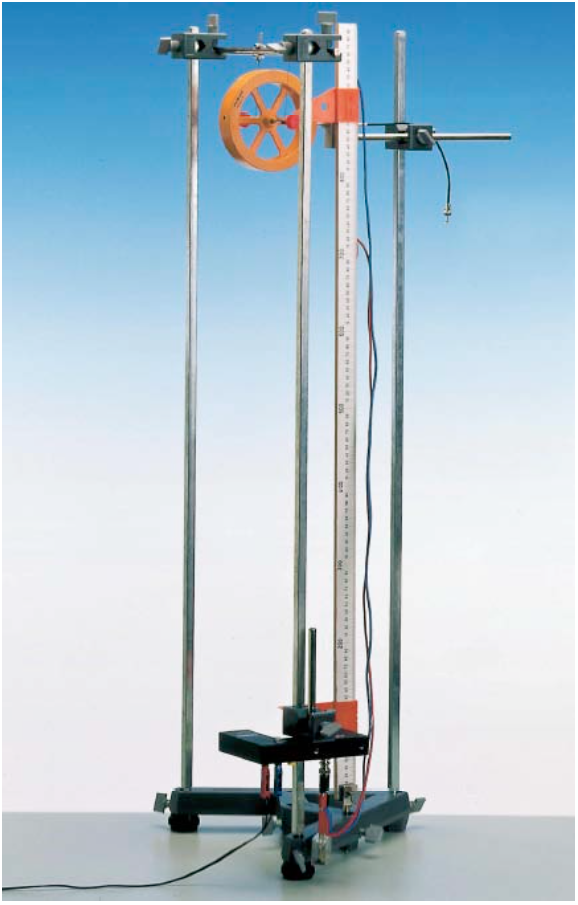
\includegraphics[width=.6\columnwidth]{maxwell.png}}
    \caption{Maxwell Wheel standart Apparatus, showing a single light barrier. Students have to carrier for each position.}
\label{figMaxwell}
\end{figure}

With this platform the small M5Stick/Arduino is attached closed to the axys anf the wheel is left to fall.
The small board, while showing the value bars on  display, and sends 
 the 6 signals of the inertial measurement unit (IMU) (speed of rotation and gravity vector 3D components). The values are stored in a InfluxDB server hosted in the Rpi. A Grafana server allow an user friendly plotting and retrieval tool, just using a plain Web Browser (``Fig.~\ref{figIMU}''). 

On an single experiment run, a simple Linear Fit on the angular velocity data, gives a very precise value of the angular acceleration,
that could be used to validate other sparse data point taken with the barrier.


\begin{figure}[htbp]
\centerline{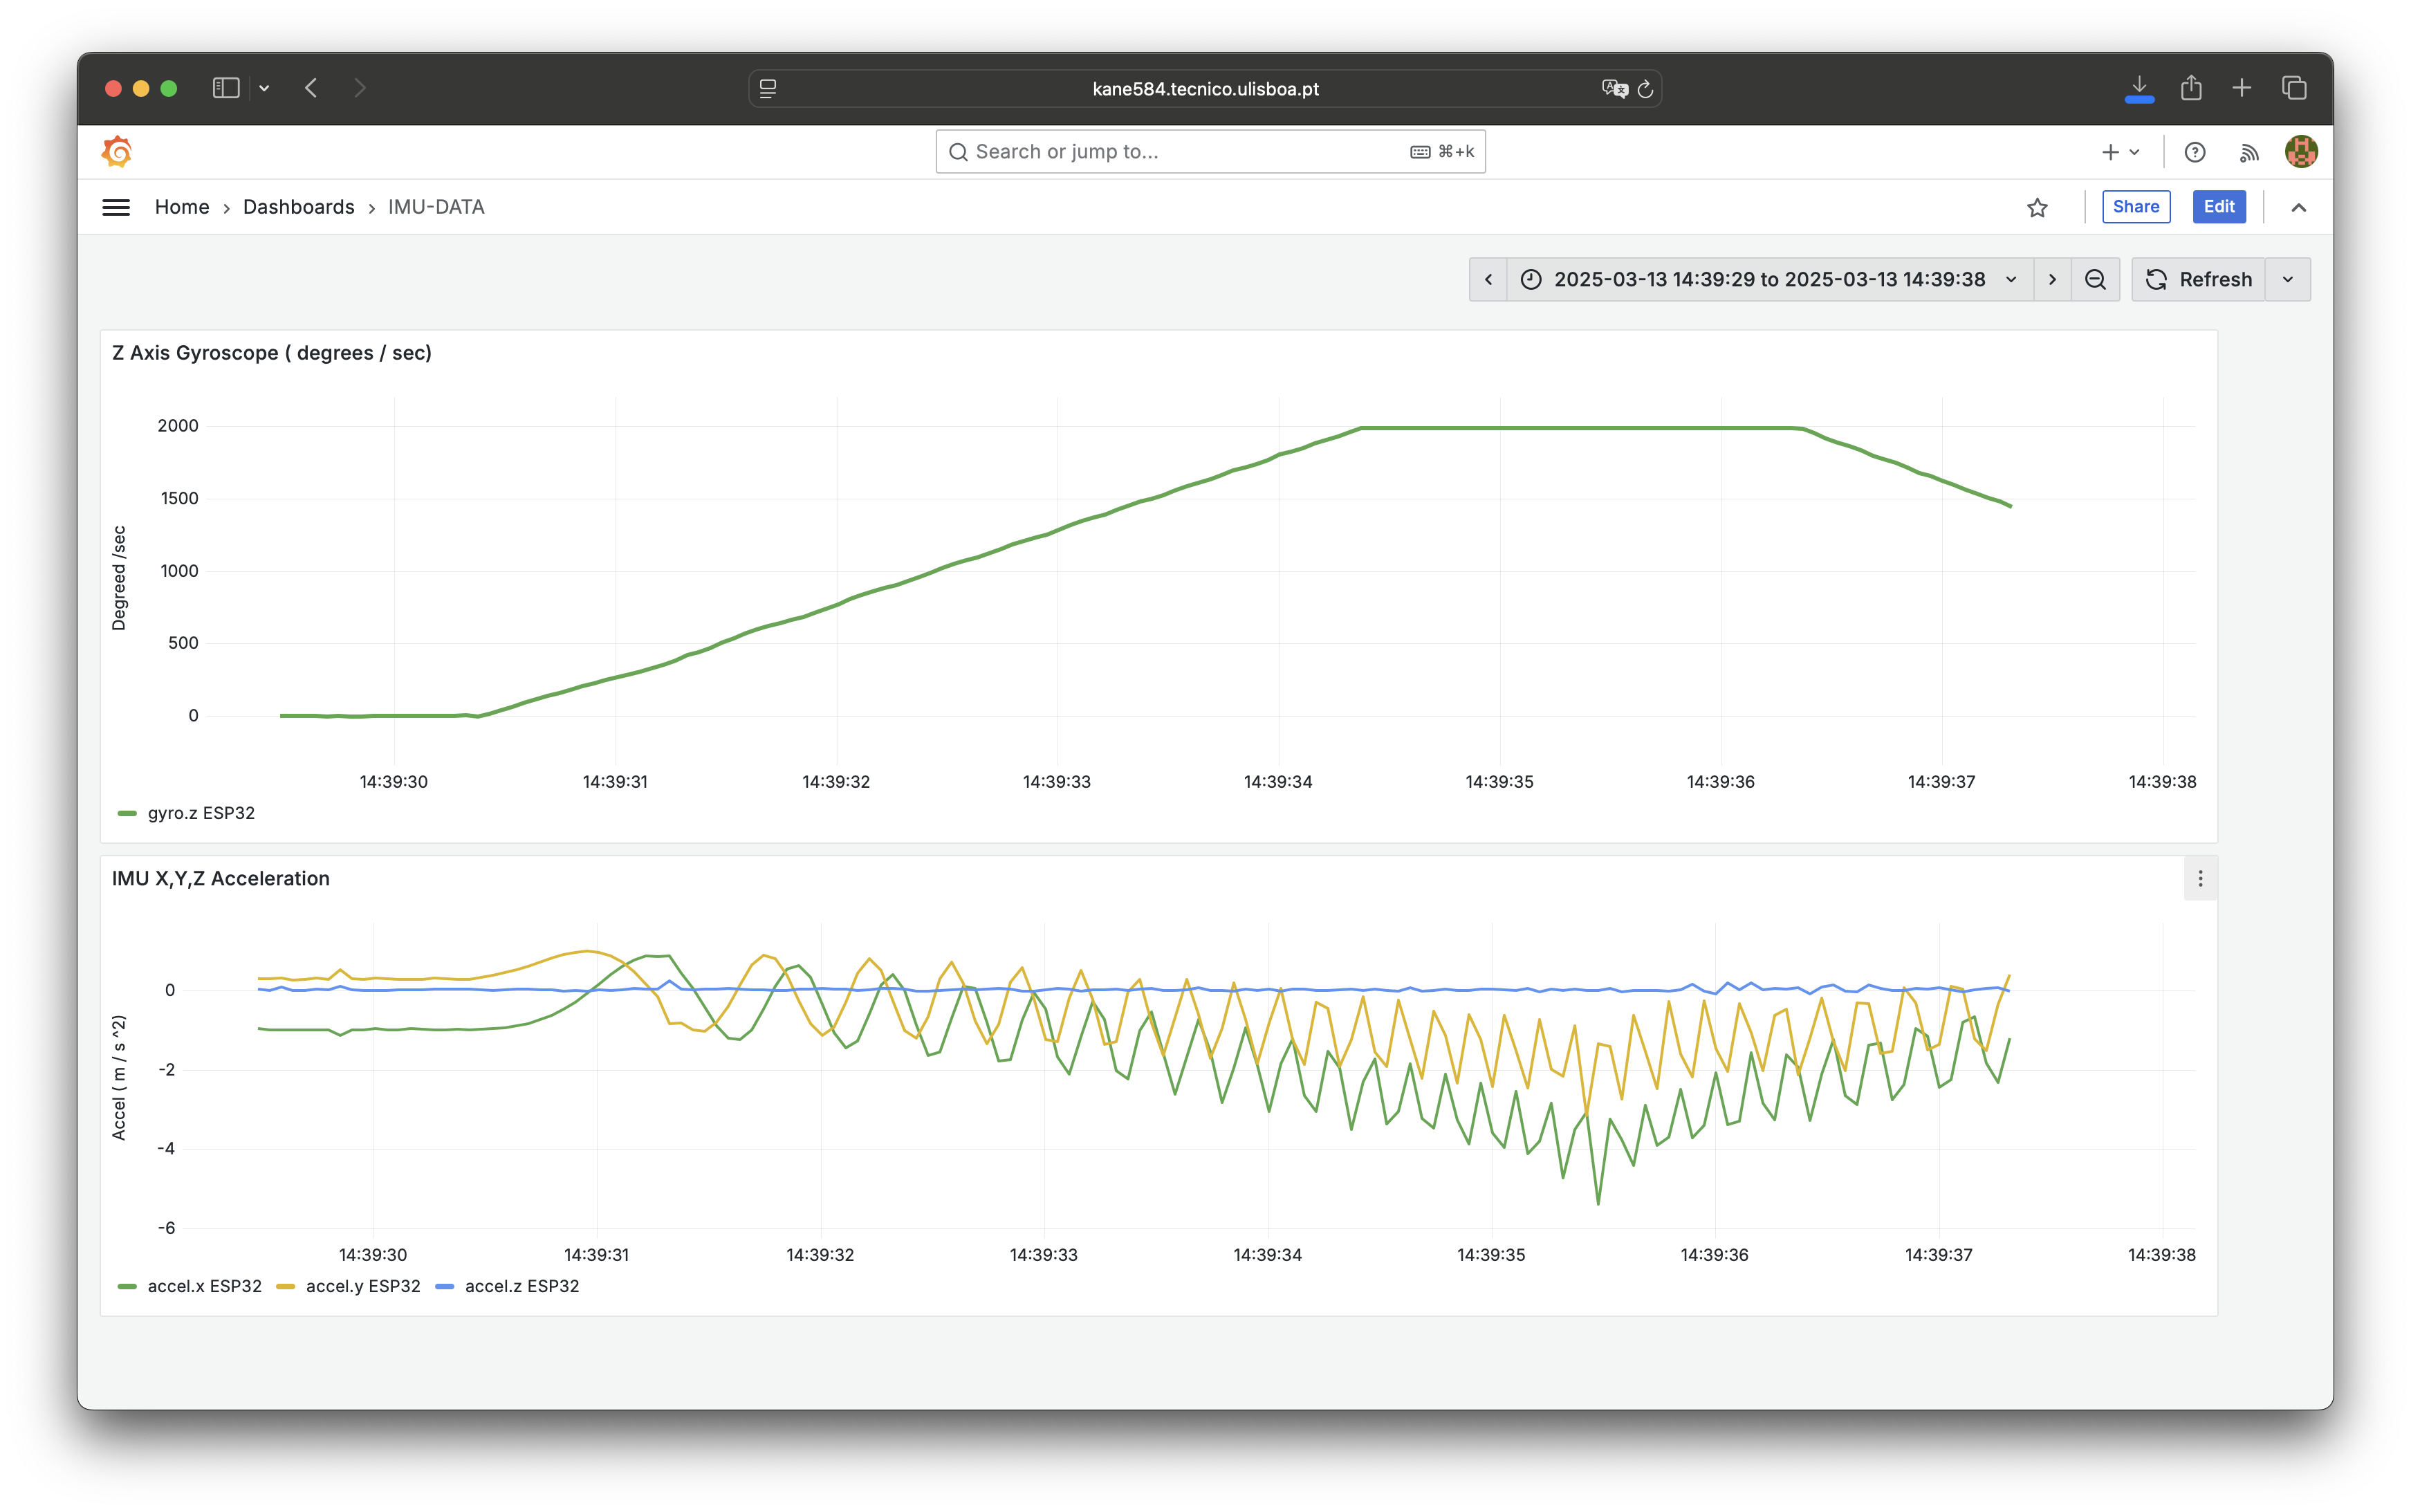
\includegraphics[width=.6\columnwidth]{IMUGrafana.png}}
\caption{Browser based plotting of rotation speed (top); and angle (bottom)of the Maxwell Wheel using Grafana}.
\label{figIMU}
\end{figure}


  
\section{Societal Impact in the Higher Teaching frame of reference}
This pedagogical project may potentially have a significant societal impact on the way teaching is conducted in higher education institutions, by bringing pinpoint capacities for simple and flexible laboratory experiments in teaching courses who may on a first approach not have considered the possibility for conducting experiments.
The tool will be implemented at Teaching Unit @ Shangai University, Spring 2025

\begin{thebibliography}{00}
\bibitem{b1}Giovanni Organtini, ``Physics Experiments with Arduino and Smartphones,''
Springer International Publishing, January 2021, DOI: 10.1007/978-3-030-65140-4.
\bibitem{b2} https://en.wikipedia.org/wiki/Arduino
\bibitem{b3} https://en.wikipedia.org/wiki/InfluxDB
\bibitem{j2} https://jupyter.org 
\bibitem{gh} https://github.com/ipfn-hpl/ard-rasp-ist
\end{thebibliography}

\end{document}
